\documentclass[12pt,a4paper]{article}

\usepackage[utf8]{inputenc}
\usepackage[T1]{fontenc}
\usepackage[spanish]{babel}
\usepackage{geometry}
\usepackage{setspace}
\usepackage{parskip}
\usepackage{enumitem}
\usepackage{booktabs}
\usepackage{array}
\usepackage{longtable}
\usepackage{tabularx}
\usepackage{multirow}
\usepackage{graphicx}
\usepackage{float}
\usepackage{amsmath}
\usepackage{amssymb}
\usepackage{caption}
\usepackage{xcolor}
\usepackage{hyperref}
\hypersetup{hidelinks}

\geometry{left=2.5cm,right=2.5cm,top=2.5cm,bottom=2.5cm}
\onehalfspacing
\graphicspath{{figuras/}}

\title{
    \textbf{Sistema de analítica y visualización para el análisis de la participación
    estudiantil en programas de internacionalización de la Universidad de los Andes}\\[0.4em]
    \large Informe técnico de avance --- Semana 9\\
    \normalsize Fase de datos: comprensión del problema, preparación de datos y análisis exploratorio
}
\author{
    Juan David Torres Albarracín\\
    Ingeniería de Sistemas y Computación\\
    Universidad de los Andes
}
\date{2026}

\begin{document}

\maketitle

\begin{abstract}
\noindent
Este informe documenta el avance del proyecto de grado hasta la semana 9 del
cronograma, correspondiente a las fases de \emph{comprensión del problema},
\emph{comprensión y preparación de datos} y \emph{análisis exploratorio} de la
metodología CRISP-DM. El objetivo del proyecto es diseñar, desarrollar y evaluar
una herramienta de analítica para la Oficina de Internacionalización que permita
explorar la participación estudiantil en programas de movilidad. En esta fase se
caracterizaron doce fuentes de datos institucionales anonimizadas, se diagnosticó
y corrigió un problema de codificación que afectaba a todas las variables de
texto, y se construyó un \textbf{pipeline reproducible} que integra las fuentes en
un conjunto de datos analítico a nivel estudiante ($233\,987$ estudiantes,
$44$ variables). La contribución metodológica central de esta fase es la
\textbf{definición de una señal de participación en internacionalización} derivada
de los registros académicos, ya que los datos no contienen una tabla explícita de
experiencias de movilidad. El análisis exploratorio sobre el subconjunto de
pregrado ($140\,422$ estudiantes, tasa de participación del $4{,}15\%$) revela una
tendencia temporal con una caída atribuible a la pandemia y recuperación
posterior, fuerte heterogeneidad por facultad y programa, un gradiente
socioeconómico y asociaciones consistentes entre participación y desempeño
académico. El informe cierra formulando la pregunta de modelamiento que se
abordará en las fases siguientes, junto con sus salvaguardas metodológicas
(manejo de desbalance e prevención de fuga de información).
\end{abstract}

\tableofcontents
\newpage

% ======================================================================
\section{Introducción y objetivo}
% ======================================================================
El proyecto propone una herramienta de analítica y visualización para que la
Oficina de Internacionalización de la Universidad de los Andes pueda explorar la
participación estudiantil en programas de movilidad e internacionalización, y
disponer de información útil para la toma de decisiones. El desarrollo sigue la
metodología CRISP-DM \cite{wirth2000,chapman2000} combinada con prácticas
iterativas de desarrollo de software.

Este documento es el informe técnico principal del proyecto y recoge, de manera
progresiva, el trabajo realizado hasta la \textbf{semana 9} del cronograma. Las
semanas 4 a 9 corresponden a las tres primeras fases de CRISP-DM:

\begin{enumerate}[leftmargin=*]
    \item \textbf{Comprensión del problema} (semana 4): usuarios, preguntas
    analíticas, alcance y criterios de éxito.
    \item \textbf{Comprensión y calidad de datos} (semanas 5--6): inventario de
    fuentes, diccionario de datos y evaluación de calidad.
    \item \textbf{Preparación de datos y análisis exploratorio} (semanas 7--9):
    pipeline de integración, definición de la señal de internacionalización,
    construcción del dataset analítico y EDA.
\end{enumerate}

El trabajo es reproducible: el código fuente del pipeline está en el paquete
\texttt{src/}, los análisis en los notebooks \texttt{notebooks/01}--\texttt{05},
y las figuras y tablas de este informe se generan automáticamente en
\texttt{reports/}. La trazabilidad de las decisiones metodológicas se concentra
en este documento (Sección~\ref{sec:trazabilidad}).

% ======================================================================
\section{Comprensión del problema (Semana 4)}
% ======================================================================
\subsection{Usuarios y preguntas analíticas}
Se identificaron tres perfiles de usuario: analistas de la Oficina (consulta y
reporte de indicadores), coordinación/dirección (planeación y comparación entre
unidades) y el equipo técnico de mantenimiento. A partir de la propuesta se
priorizaron siete preguntas analíticas (PA):

\begin{description}[leftmargin=1.4cm,style=nextline]
    \item[PA1] Evolución temporal de la participación.
    \item[PA2] Participación por facultad y programa académico.
    \item[PA3] Modalidades de movilidad más frecuentes.
    \item[PA4] Momento de la trayectoria académica en que ocurre la movilidad.
    \item[PA5] Características académicas asociadas a la participación.
    \item[PA6] Diferencias entre grupos (género, estrato, tipo de admisión).
    \item[PA7] Estimación de la probabilidad de participación (modelamiento).
\end{description}

\subsection{Alcance y criterios de éxito de la fase}
El alcance de la fase de datos comprende: un dataset analítico documentado y
reproducible, la definición justificada de la señal de internacionalización, un
informe de calidad de datos, un EDA que responda PA1--PA6 y la formulación de la
pregunta de modelamiento (PA7). El detalle de requerimientos funcionales y no
funcionales se encuentra en \texttt{docs/01\_requerimientos\_semana4.md}.

% ======================================================================
\section{Comprensión y calidad de los datos (Semanas 5--6)}
% ======================================================================
\subsection{Inventario de fuentes}
Se dispone de doce archivos \texttt{parquet} anonimizados. La
Tabla~\ref{tab:fuentes} resume las fuentes núcleo utilizadas en esta fase, su
tamaño y granularidad. Todas identifican al estudiante mediante un código
anonimizado; dos fuentes grandes usan el sufijo \texttt{\_ANOM}, lo que se
normaliza en el pipeline.

\begin{table}[H]
\centering
\caption{Fuentes núcleo del proyecto y su granularidad.}
\label{tab:fuentes}
\small
\begin{tabular}{>{\raggedright\arraybackslash}p{4.6cm} r r >{\raggedright\arraybackslash}p{4.6cm}}
\toprule
\textbf{Fuente} & \textbf{Filas} & \textbf{Variables} & \textbf{Unidad de información} \\
\midrule
informacion\_actual        & 233\,987   & 73 & Estudiante (snapshot, 1 fila/estudiante) \\
historial\_materias        & 6\,958\,732 & 14 & Curso--estudiante--periodo \\
programas                  & 1\,770\,486 & 18 & Programa--estudiante--periodo \\
historial\_rendimiento     & 1\,230\,195 & 28 & Estudiante--periodo \\
percentiles\_historicos    & 994\,875   & 18 & Estudiante--periodo \\
icfes\_saber11             & 262\,148   & 10 & Presentación de examen \\
grados                     & 139\,429   & 10 & Grado obtenido \\
historial\_opciones        & 173\,387   & 14 & Opción--estudiante--periodo \\
examenes\_clasificacion    & 79\,599    & 8  & Clasificación por estudiante \\
capp\_creditos             & 30\,771    & 7  & Cálculo de créditos \\
\bottomrule
\end{tabular}
\end{table}

\textbf{Decisión (unidad de análisis).} Se adopta el \emph{estudiante} como unidad
de análisis y \texttt{informacion\_actual} (una fila por estudiante) como columna
vertebral; las fuentes transaccionales se agregan a nivel estudiante. El
diccionario de datos completo se exporta en
\texttt{reports/tables/diccionario\_datos.csv}.

\subsection{Calidad de datos y codificación}
\label{sec:calidad}
El perfilamiento (notebook \texttt{02}) identificó cuatro problemas de calidad y
las decisiones correspondientes:

\paragraph{1. Codificación (\emph{mojibake}).} Todas las columnas de texto
presentaban caracteres corruptos. Se diagnosticaron \textbf{dos esquemas
distintos}: en \texttt{informacion\_actual} el texto UTF-8 fue interpretado con
CP437 (p.\,ej. \emph{Magíster} aparecía como \texttt{Mag}+símbolo y \emph{Opción}
con un símbolo en lugar de la ``ó''); en \texttt{historial\_materias} fue
interpretado con CP850 (p.\,ej. \emph{DOBLE TITULACIÓN} y \emph{PRÁCTICA} con
símbolos de caja en lugar de las vocales acentuadas). Se implementó una corrección
automática que detecta el esquema aplicable y recupera el texto en español
(\emph{Magíster}, \emph{Opción}, \emph{DOBLE TITULACIÓN}, \emph{PRÁCTICA}).
\textbf{Esta corrección es imprescindible}: sin ella, categorías idénticas se
contarían como distintas.

\paragraph{2. Valores faltantes.} Variables socioeconómicas y de ingreso
presentan ausencias elevadas, en parte por la heterogeneidad del snapshot
(estudiantes antiguos sin ICFES moderno, trayectorias cortas sin rendimiento
consolidado). No se descartan a priori; se evalúa su cobertura en el subconjunto
de pregrado (Sección~\ref{sec:faltantes}).

\paragraph{3. Múltiples filas por estudiante} en ICFES, CAPP y exámenes. Se adopta
una regla de deduplicación explícita: para ICFES, el registro de mayor puntaje
total; para CAPP y exámenes, el más reciente por fecha.

\paragraph{4. Valores atípicos.} El PGA se encuentra dentro del rango esperado
$[0,5]$; los valores bajos (incluidos ceros) corresponden a inicios de
trayectoria y se conservan.

El informe de calidad completo está en
\texttt{reports/tables/informe\_calidad\_datos.csv}.

% ======================================================================
\section{Preparación de datos (Semanas 7--8)}
% ======================================================================
\subsection{Definición de la señal de internacionalización}
\label{sec:senal}
Las fuentes entregadas \textbf{no contienen una tabla explícita de experiencias
de internacionalización}. Por lo tanto, la participación debe \emph{derivarse} de
los registros académicos. Esta es la decisión metodológica central de la fase de
datos.

\textbf{Criterio adoptado.} La Universidad inscribe las experiencias de movilidad
como asignaturas en la historia académica del estudiante
(\texttt{historial\_materias}). Se marca un registro como \emph{evento de
movilidad} cuando el nombre del curso (corregido de encoding) coincide con un
patrón de movilidad --- \texttt{INTERCAMBIO}, \texttt{VIAJE INTERNACIONAL},
\texttt{SEMANA INTERNACIONAL}, \texttt{DOBLE TITULAC} --- o cuando su código
pertenece a una lista canónica de cursos de movilidad (p.\,ej. \texttt{DECA-2201},
\texttt{INTL-2201}, \texttt{MBAE-4543}). Cada evento se clasifica en una
\emph{modalidad}.

\textbf{Justificación.} (i)~Se usa el nombre del curso \emph{además} del código
porque una misma experiencia aparece bajo múltiples códigos de departamento;
confiar solo en códigos subestimaría la señal. (ii)~Se excluye la modalidad
``intercambio nacional'' del foco internacional mediante un parámetro explícito.
(iii)~La señal se construye sin mirar ninguna variable posterior al evento, de
modo que pueda reutilizarse como variable objetivo en el modelamiento sin
introducir fuga de información. La definición está implementada y es auditable en
\texttt{src/internationalization.py}.

La Tabla~\ref{tab:modalidades} y la Figura~\ref{fig:modalidades} resumen la
composición de la señal.

\begin{table}[H]
\centering
\caption{Composición de la señal de internacionalización por modalidad (eventos).}
\label{tab:modalidades}
\small
\begin{tabular}{l r}
\toprule
\textbf{Modalidad} & \textbf{Eventos} \\
\midrule
Intercambio internacional        & 7\,726 \\
Doble titulación                 & 817 \\
Viaje internacional de estudio   & 559 \\
Semana internacional             & 396 \\
Intercambio virtual              & 28 \\
\midrule
\textbf{Total}                   & \textbf{9\,526} \\
\bottomrule
\end{tabular}
\end{table}

\begin{figure}[H]
\centering
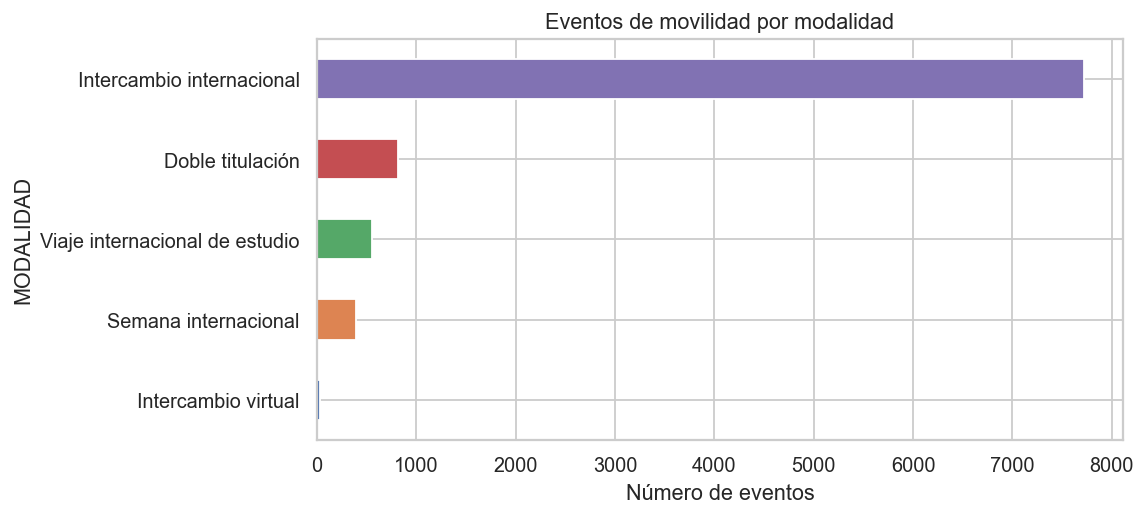
\includegraphics[width=0.72\textwidth]{fig_modalidades_eventos.png}
\caption{Eventos de movilidad por modalidad. El intercambio internacional
concentra cerca del 81\% de los eventos.}
\label{fig:modalidades}
\end{figure}

\subsection{Construcción del dataset analítico}
El pipeline (\texttt{src/build\_dataset.py}, ejecutable con
\texttt{python -m src.build\_dataset}) integra las fuentes mediante uniones por la
izquierda sobre la columna vertebral, de modo que no se pierden estudiantes del
universo. Agrega el desempeño académico (PGA histórico y último, créditos,
semestres), la posición relativa (percentil de PGA), el avance (semestre), las
pruebas de ingreso (ICFES), la clasificación de inglés/matemáticas, el progreso de
créditos (CAPP) y la etiqueta \texttt{PARTICIPA}. El resultado es un dataset de
\textbf{$233\,987$ estudiantes $\times$ $44$ variables}, validado automáticamente
(clave única, conservación del universo, etiqueta binaria).

\textbf{Prevención de fuga de información.} El pipeline conserva, por estudiante,
el primer periodo de movilidad (\texttt{PRIMER\_PERIODO\_MOVILIDAD}). En la fase de
modelamiento, los predictores de desempeño deberán calcularse en un corte
temporal anterior a ese periodo, en coherencia con la advertencia de la propuesta
sobre \emph{data leakage}.

\subsection{Desbalance de clases}
La participación es un fenómeno minoritario: \textbf{$3{,}43\%$ global} y
\textbf{$4{,}15\%$ en pregrado}. El pregrado concentra el mayor volumen de
participantes ($5\,821$) y la tasa más alta entre los niveles con volumen
relevante, lo que motiva centrar el análisis y el modelamiento en este nivel.

\subsection{Tratamiento de valores faltantes}
\label{sec:faltantes}
En el subconjunto de pregrado, la cobertura de las variables candidatas es:
\texttt{NIVEL\_INGLES} $\approx 12\%$ (faltante $87{,}8\%$), bloque de
PGA/percentil/avance $\approx 45$--$55\%$ de faltante, e ICFES $\approx 45\%$ de
faltante. Decisiones:

\begin{itemize}[leftmargin=*]
    \item \texttt{NIVEL\_INGLES} se \textbf{descarta} como variable principal por
    cobertura insuficiente; se conserva el puntaje de inglés del ICFES.
    \item Para las variables de desempeño e ICFES se adoptará, en el
    modelamiento, \textbf{imputación por mediana más un indicador de faltante},
    evitando descartar estudiantes y haciendo explícito el mecanismo del faltante,
    en línea con la literatura \cite{little2019}. No se imputa en el EDA: aquí se
    analizan los datos observados.
\end{itemize}

% ======================================================================
\section{Análisis exploratorio (Semanas 8--9)}
% ======================================================================
\subsection{Panorama univariado}
La Figura~\ref{fig:univcat} muestra la distribución de variables categóricas en
pregrado. La población se concentra en pocas facultades grandes (Ingeniería es la
de mayor volumen), con género relativamente equilibrado y fuerte presencia de
estratos 3--6; una fracción no despreciable tiene estrato ausente. La
Figura~\ref{fig:univnum} confirma escalas coherentes: PGA concentrado en
$3{,}8$--$4{,}0$, percentil aproximadamente uniforme e ICFES aproximadamente
simétrico alrededor de $\sim 355$.

\begin{figure}[H]
\centering
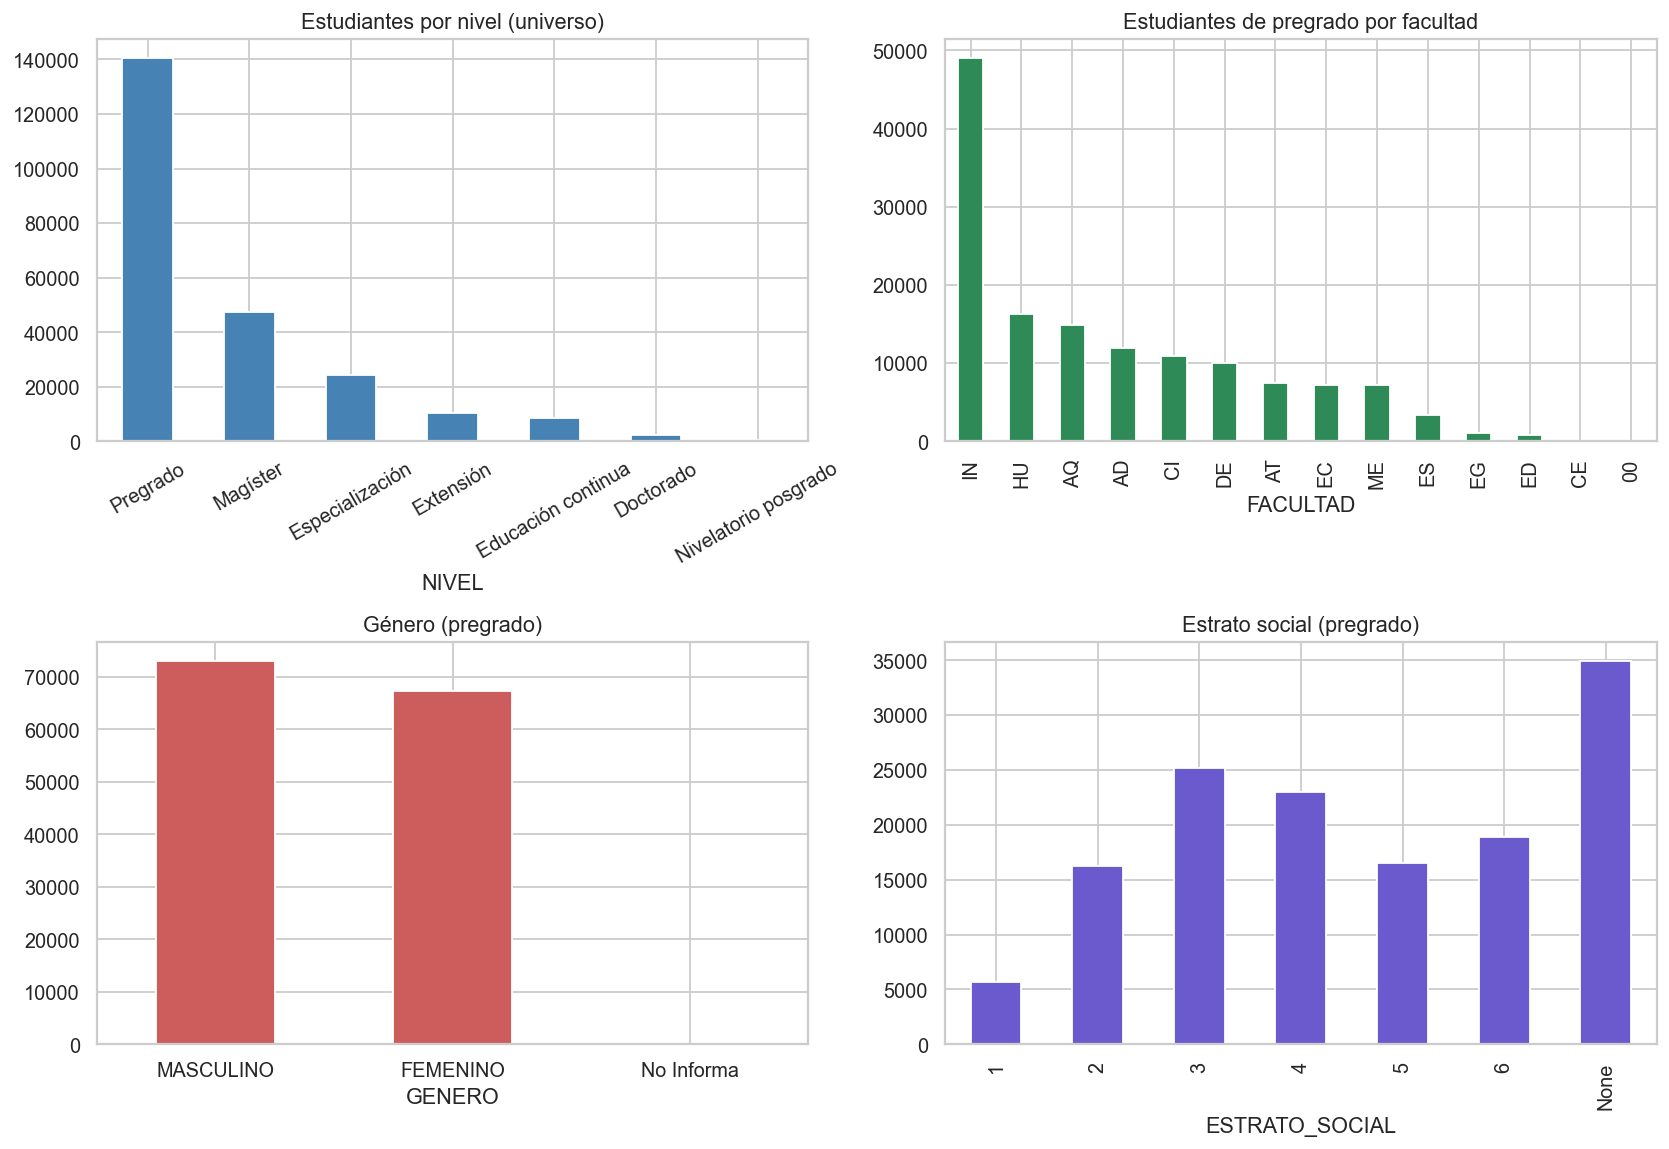
\includegraphics[width=0.92\textwidth]{fig_univariado_categoricas.png}
\caption{Distribuciones univariadas de variables categóricas (pregrado).}
\label{fig:univcat}
\end{figure}

\begin{figure}[H]
\centering
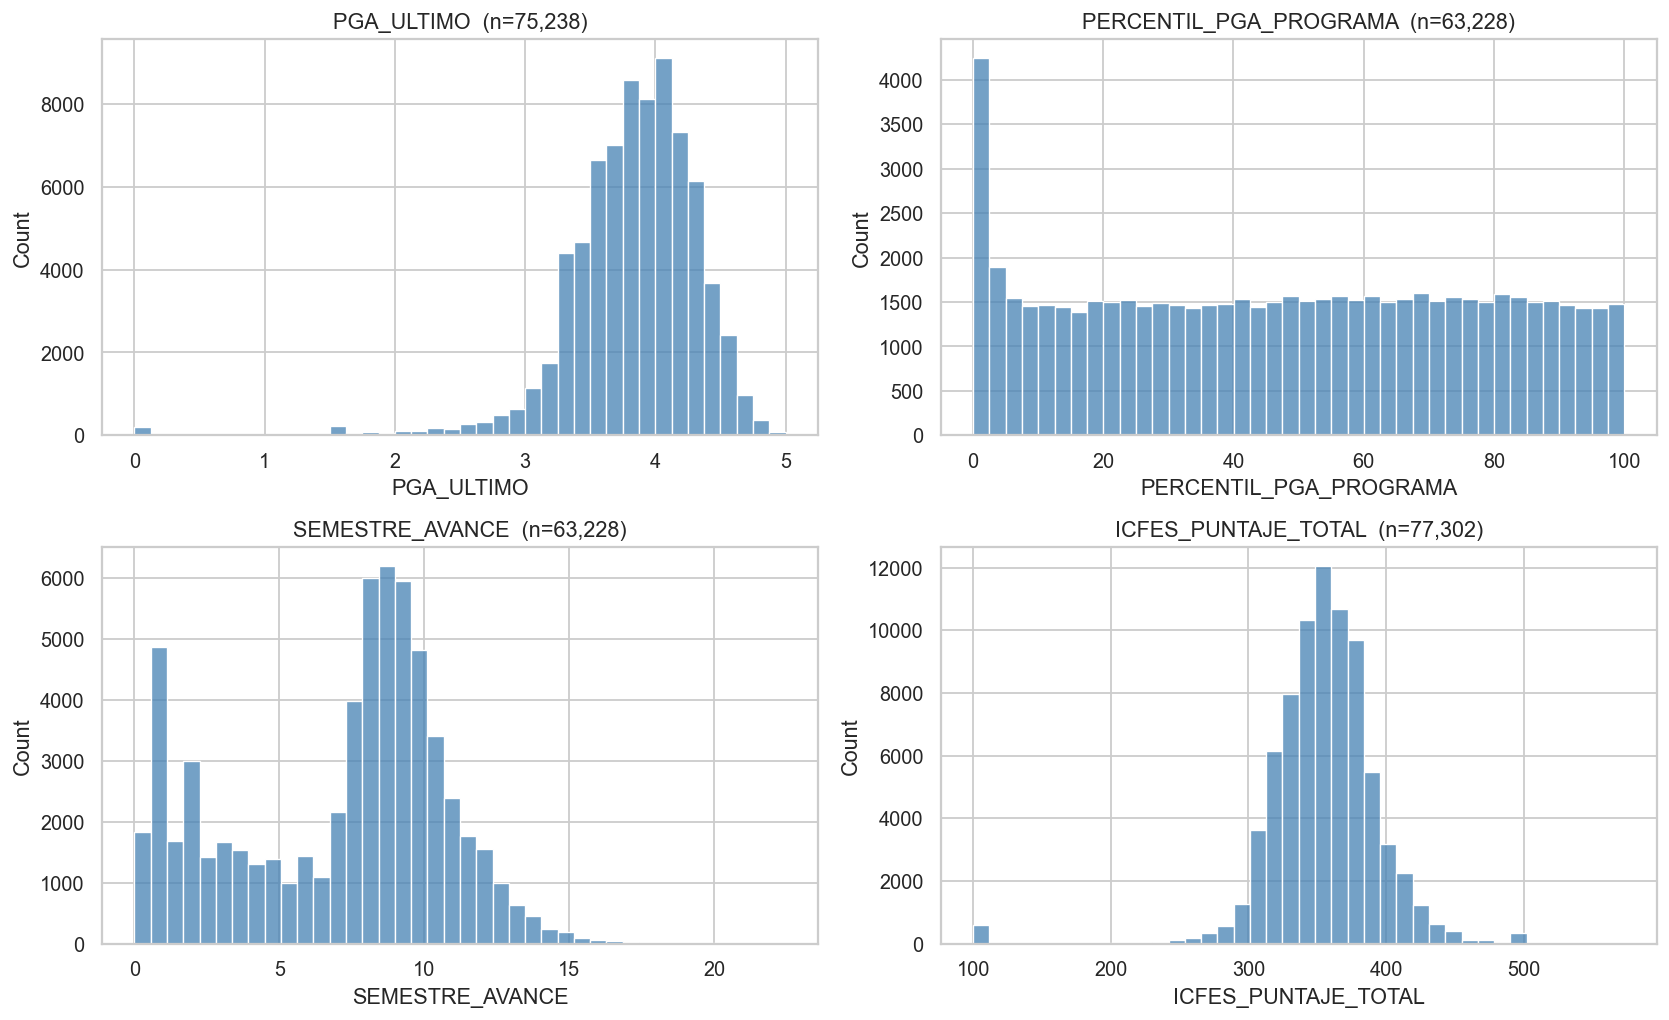
\includegraphics[width=0.92\textwidth]{fig_univariado_numericas.png}
\caption{Distribuciones univariadas de variables numéricas de desempeño e ingreso
(pregrado).}
\label{fig:univnum}
\end{figure}

\subsection{PA1 --- Evolución temporal}
La Figura~\ref{fig:temporal} muestra una tendencia creciente de la movilidad
hasta estabilizarse en $\sim 400$--$450$ eventos anuales en la década de 2010, una
\textbf{caída pronunciada en 2020--2021} ($447$ eventos en 2019 frente a $257$ y
$268$ en 2020 y 2021) atribuible a las restricciones de la pandemia de COVID-19, y
una \textbf{recuperación fuerte desde 2022} que alcanza máximos históricos
($\sim 585$--$595$ eventos en 2023--2025). Que la señal reaccione a un choque
externo conocido de la forma esperada es también una validación indirecta de su
correcta construcción.

\begin{figure}[H]
\centering
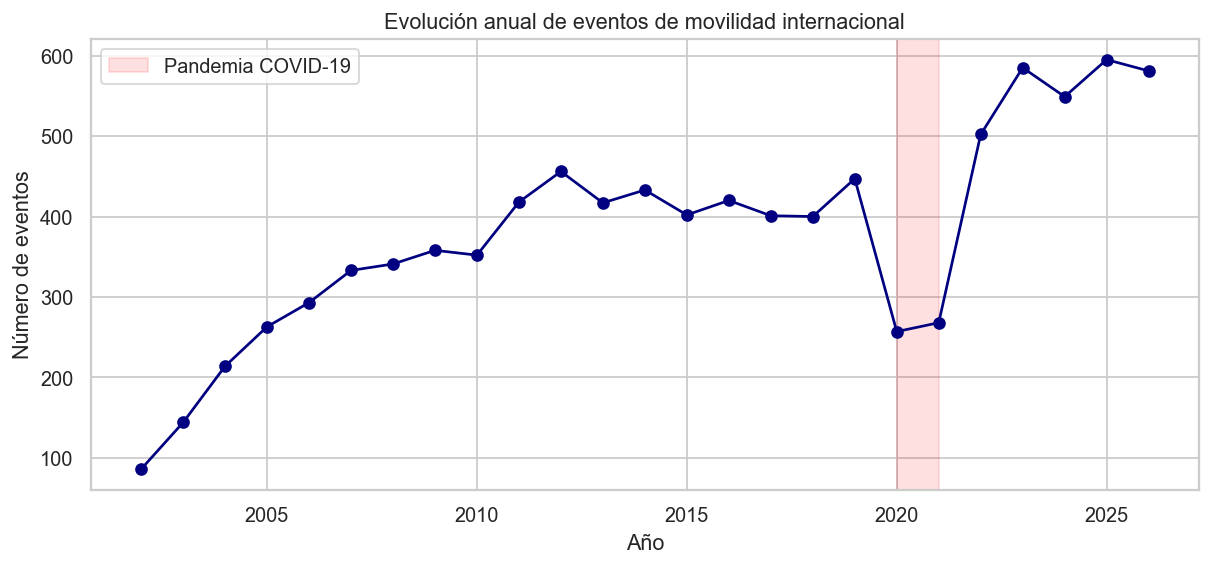
\includegraphics[width=0.92\textwidth]{fig_evolucion_temporal.png}
\caption{Evolución anual de eventos de movilidad internacional. La franja roja
señala el periodo de pandemia.}
\label{fig:temporal}
\end{figure}

\subsection{PA3 --- Modalidades en el tiempo}
La Figura~\ref{fig:modtemporal} muestra que el intercambio internacional domina
en todo el periodo, con contribuciones menores pero estables de doble titulación,
viajes y semanas internacionales. El intercambio virtual aparece puntualmente
alrededor de 2020--2021, coherente con la sustitución de la movilidad física
durante la pandemia.

\begin{figure}[H]
\centering
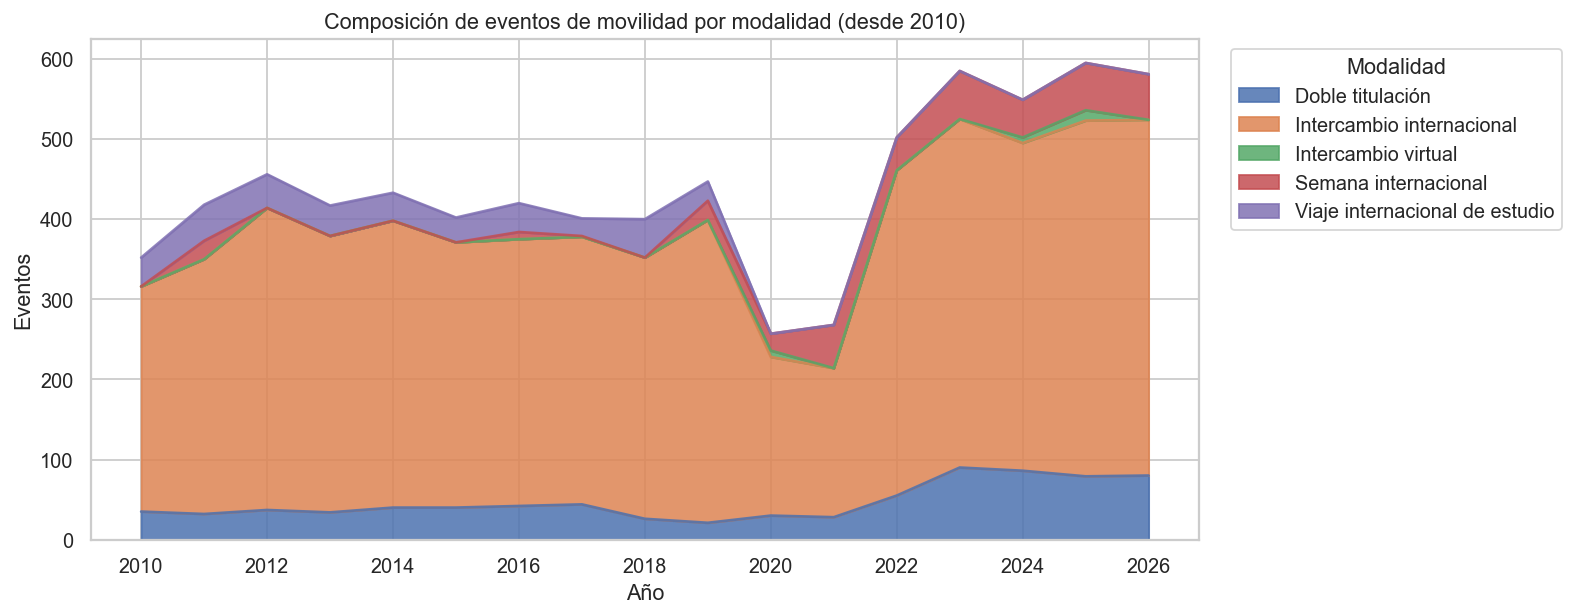
\includegraphics[width=0.92\textwidth]{fig_modalidad_temporal.png}
\caption{Composición de eventos de movilidad por modalidad desde 2010.}
\label{fig:modtemporal}
\end{figure}

\subsection{PA2 --- Participación por facultad y programa}
La participación es muy heterogénea entre unidades académicas
(Figura~\ref{fig:facultad}): la tasa va desde $\sim 0{,}1\%$ hasta
$\sim 12{,}3\%$ (Administración presenta la tasa más alta; Arquitectura, Economía
y Derecho también destacan). A nivel de programa (Figura~\ref{fig:programa}) la
heterogeneidad es aún mayor. La facultad/programa es, por tanto, una variable
estructural clave y una dimensión de segmentación prioritaria para el dashboard.

\begin{figure}[H]
\centering
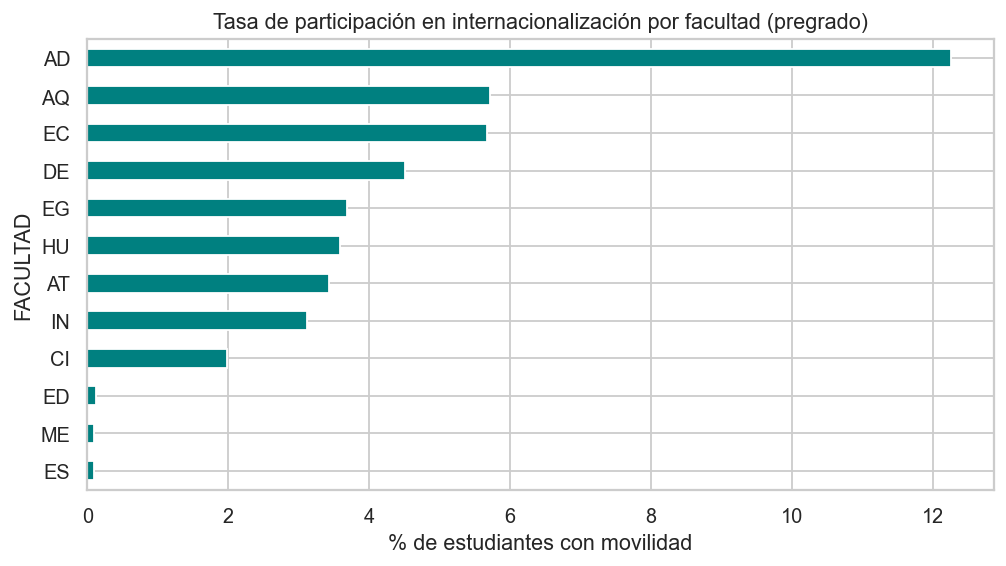
\includegraphics[width=0.80\textwidth]{fig_tasa_por_facultad.png}
\caption{Tasa de participación por facultad (pregrado).}
\label{fig:facultad}
\end{figure}

\begin{figure}[H]
\centering
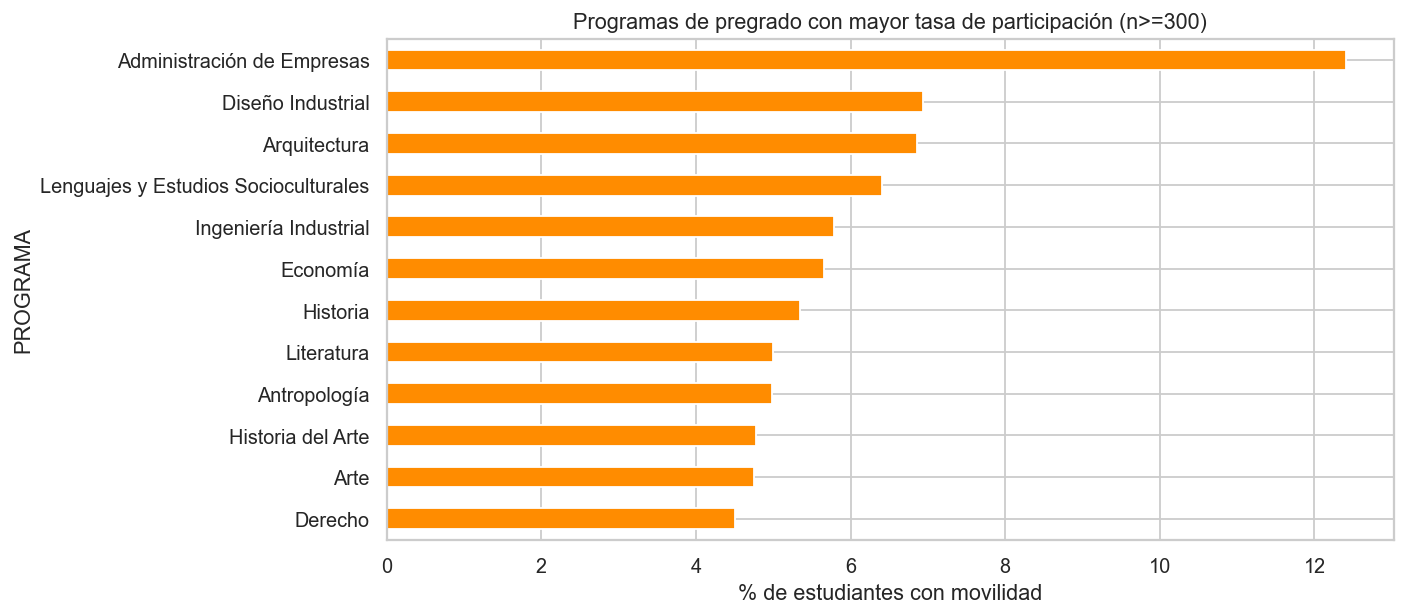
\includegraphics[width=0.82\textwidth]{fig_tasa_por_programa.png}
\caption{Programas de pregrado con mayor tasa de participación
($n \geq 300$).}
\label{fig:programa}
\end{figure}

\subsection{PA4 --- Momento de la trayectoria}
Los participantes se concentran en etapas intermedias y avanzadas de la carrera
(Figura~\ref{fig:momento}): su avance mediano es de $\sim 8{,}75$ semestres frente
a $\sim 8$ en no participantes, con una distribución mucho más estrecha. Esto
tiene una implicación directa sobre el modelamiento: los predictores de desempeño
deben ``congelarse'' en un corte anterior al primer evento, no al final de la
trayectoria.

\begin{figure}[H]
\centering
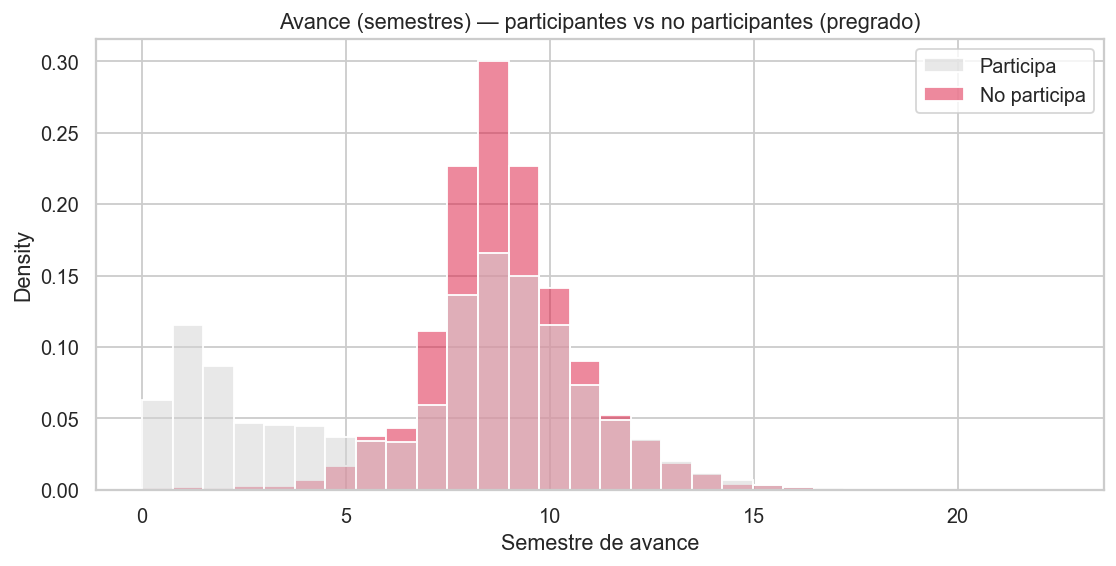
\includegraphics[width=0.85\textwidth]{fig_momento_trayectoria.png}
\caption{Avance en semestres: participantes frente a no participantes (pregrado).}
\label{fig:momento}
\end{figure}

\subsection{PA5--PA6 --- Perfil académico y diferencias entre grupos}
Los participantes muestran, en promedio, mejor desempeño y mejor perfil de ingreso
(Figura~\ref{fig:bivdesempeno}, Tabla~\ref{tab:perfil}). Existe además un
\textbf{gradiente socioeconómico} claro (Tabla~\ref{tab:grupos}): la tasa de
participación crece de forma monótona con el estrato (de $\sim 0{,}4\%$ en estratos
1--2 a $\sim 9{,}5\%$ en estrato 6) y es algo mayor en mujeres. Estos resultados
deben interpretarse como \textbf{asociaciones, no causas}, y comunicarse como
análisis de equidad.

\begin{figure}[H]
\centering
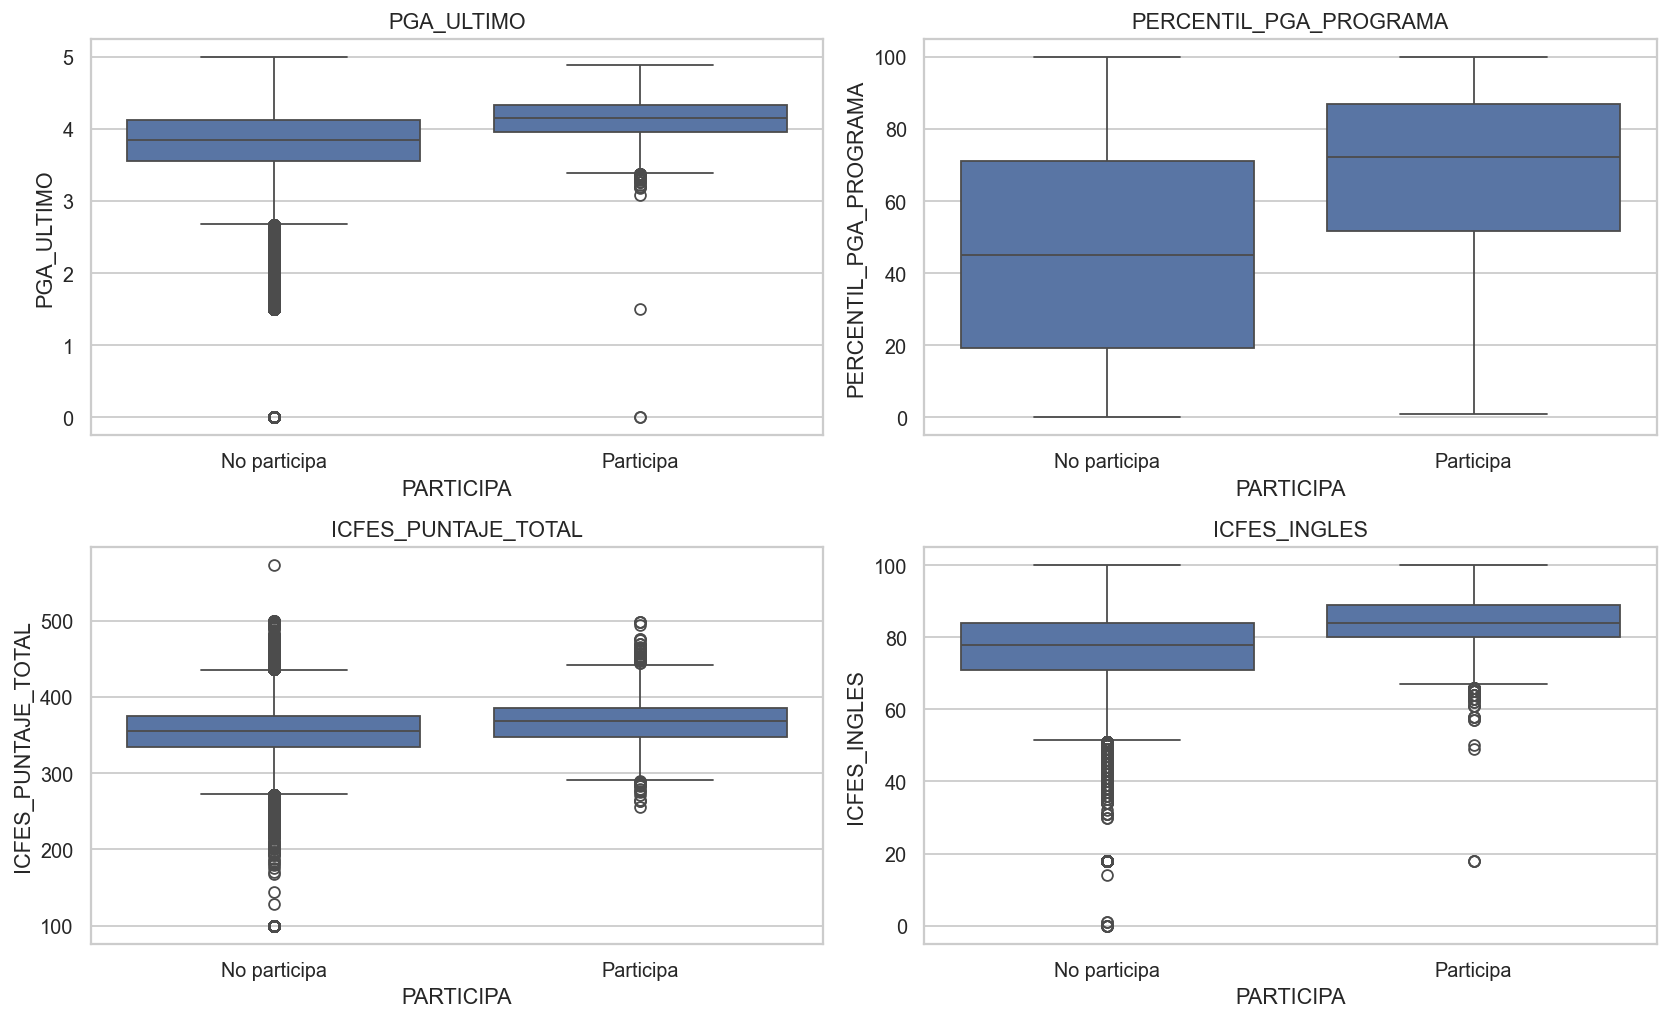
\includegraphics[width=0.92\textwidth]{fig_bivariado_desempeno.png}
\caption{Comparación del desempeño y perfil de ingreso entre participantes y no
participantes (pregrado).}
\label{fig:bivdesempeno}
\end{figure}

\begin{table}[H]
\centering
\caption{Perfil promedio de participantes y no participantes (pregrado).}
\label{tab:perfil}
\small
\begin{tabular}{l r r r}
\toprule
\textbf{Variable} & \textbf{No participa} & \textbf{Participa} & \textbf{Diferencia} \\
\midrule
PGA (último)                 & 3{,}81 & 4{,}14 & $+0{,}33$ \\
Percentil PGA (programa)     & 45{,}8 & 67{,}7 & $+21{,}9$ \\
Semestre de avance           & 6{,}93 & 8{,}87 & $+1{,}95$ \\
ICFES total                  & 354{,}3 & 368{,}4 & $+14{,}1$ \\
ICFES inglés                 & 77{,}4 & 84{,}6 & $+7{,}2$ \\
\% créditos aprobados        & 0{,}86 & 0{,}94 & $+0{,}09$ \\
\bottomrule
\end{tabular}
\end{table}

\begin{table}[H]
\centering
\caption{Tasa de participación por grupo (pregrado).}
\label{tab:grupos}
\small
\begin{tabular}{l r l r}
\toprule
\multicolumn{2}{c}{\textbf{Estrato social}} & \multicolumn{2}{c}{\textbf{Género}} \\
\textbf{Estrato} & \textbf{Tasa (\%)} & \textbf{Género} & \textbf{Tasa (\%)} \\
\midrule
6 & 9{,}48 & Femenino  & 4{,}65 \\
5 & 6{,}26 & Masculino & 3{,}68 \\
4 & 3{,}33 &           &        \\
3 & 0{,}94 &           &        \\
2 & 0{,}43 &           &        \\
1 & 0{,}42 &           &        \\
\bottomrule
\end{tabular}
\end{table}

\subsection{Asociación multivariada}
La Figura~\ref{fig:corr} presenta las correlaciones entre variables numéricas y
la participación. Individualmente, las correlaciones con \texttt{PARTICIPA} son de
magnitud baja a moderada (lo esperable para un evento poco frecuente), pero con
signos coherentes: el percentil de PGA por programa y el PGA muestran la
asociación positiva más clara, seguidos del avance y el perfil de ingreso. Ninguna
variable domina por sí sola, lo que anticipa que un modelo multivariado --- y
posiblemente no lineal --- capturará mejor el fenómeno que cualquier regla
univariada. La correlación entre predictores (p.\,ej. PGA y percentil) alerta
sobre colinealidad a considerar en modelos lineales.

\begin{figure}[H]
\centering
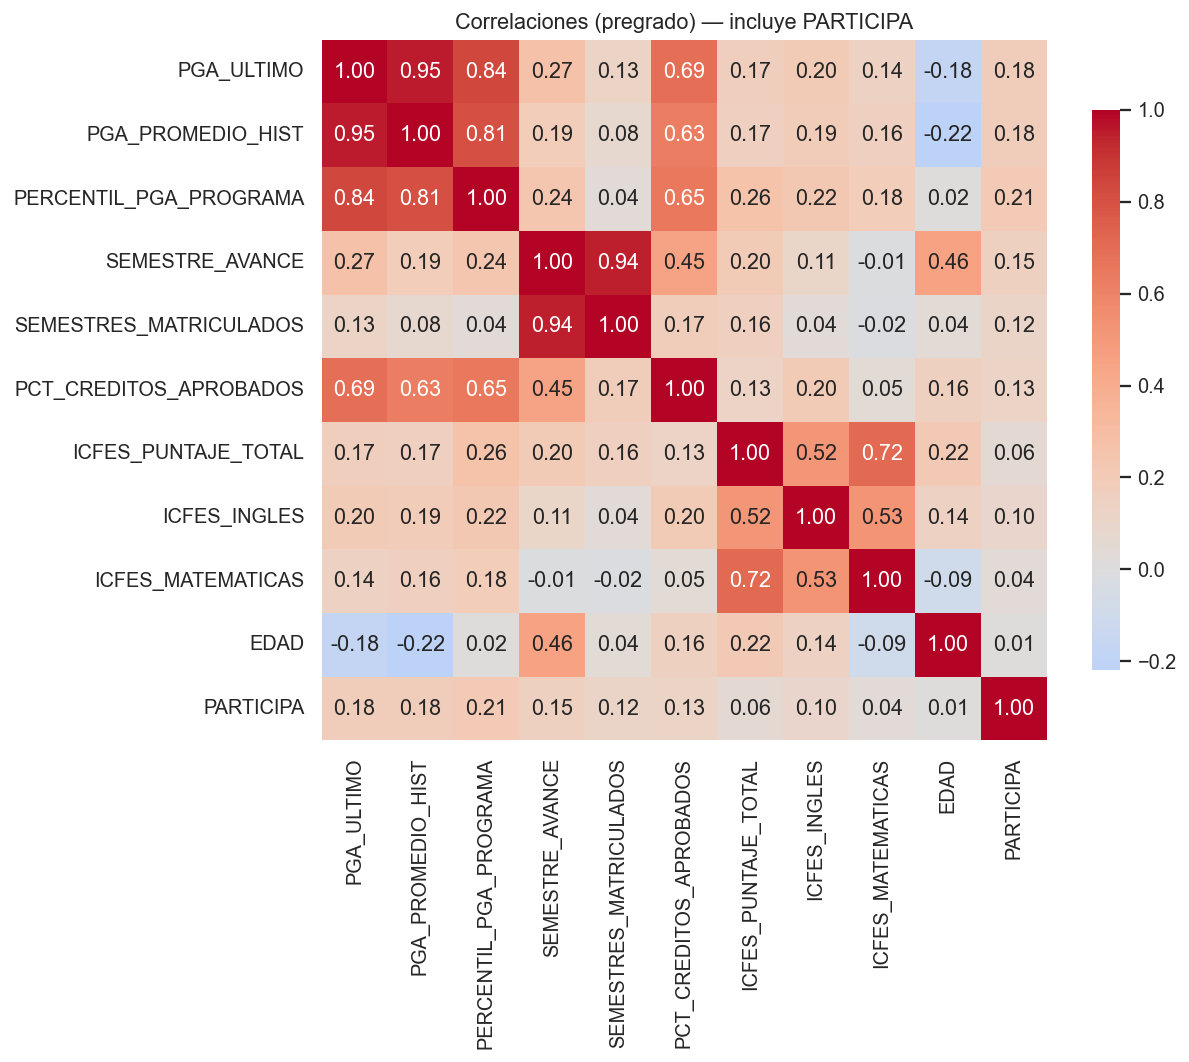
\includegraphics[width=0.80\textwidth]{fig_correlaciones.png}
\caption{Matriz de correlaciones de variables numéricas (pregrado), incluyendo la
etiqueta de participación.}
\label{fig:corr}
\end{figure}

\subsection{Indicadores principales}
La Tabla~\ref{tab:indicadores} consolida los indicadores que alimentarán el módulo
de resumen del dashboard (exportados en
\texttt{reports/tables/indicadores\_principales.csv}).

\begin{table}[H]
\centering
\caption{Indicadores principales de la fase de datos.}
\label{tab:indicadores}
\small
\begin{tabular}{l r}
\toprule
\textbf{Indicador} & \textbf{Valor} \\
\midrule
Estudiantes (universo)                 & 233\,987 \\
Estudiantes de pregrado                & 140\,422 \\
Participantes (total)                  & 8\,036 \\
Participantes (pregrado)               & 5\,821 \\
Tasa de participación global           & 3{,}43\% \\
Tasa de participación en pregrado      & 4{,}15\% \\
Eventos de movilidad                   & 9\,526 \\
Año pico de eventos                    & 2025 \\
Modalidad principal                    & Intercambio internacional \\
Facultad con mayor tasa                & Administración \\
Avance mediano de participantes        & 8{,}75 semestres \\
\bottomrule
\end{tabular}
\end{table}

% ======================================================================
\section{Formulación del problema de modelamiento (PA7)}
% ======================================================================
A partir del análisis se formaliza el problema que se abordará desde la semana 10:

\begin{quote}
\textit{Dado un estudiante de pregrado, estimar la probabilidad de que participe
en una experiencia de internacionalización en algún momento de su carrera, usando
únicamente información disponible antes del evento.}
\end{quote}

\textbf{Justificación.} Existe una variable objetivo bien definida y auditable
(\texttt{PARTICIPA}) con una tasa de base realista; el EDA mostró asociaciones
consistentes que dan sustento a un modelo con capacidad discriminante; y el
problema es relevante para la Oficina, pues permite identificar perfiles con baja
participación y focalizar estrategias.

\textbf{Salvaguardas metodológicas heredadas al modelamiento.}
\begin{enumerate}[leftmargin=*]
    \item \emph{Desbalance de clases}: la exactitud no basta (un clasificador
    trivial acertaría $\sim 96\%$); se usarán precisión, \emph{recall}, F1 y
    PR-AUC, además de ROC-AUC, y se evaluarán técnicas de manejo de desbalance
    \cite{saito2015}.
    \item \emph{Prevención de fuga de información}: los predictores se calcularán
    en un corte temporal anterior al primer evento de movilidad.
    \item \emph{Complejidad progresiva}: línea base trivial, regresión logística
    \cite{hastie2009}, árboles/Random Forest \cite{breiman2001}, boosting
    \cite{chen2016}, con interpretabilidad mediante SHAP \cite{lundberg2017} y
    validación cruzada \cite{kohavi1995}. Las implementaciones se apoyarán en
    \emph{scikit-learn} \cite{pedregosa2011}.
    \item \emph{Variables descartadas} por cobertura: \texttt{NIVEL\_INGLES}.
\end{enumerate}

% ======================================================================
\section{Trazabilidad de decisiones metodológicas}
\label{sec:trazabilidad}
% ======================================================================
La Tabla~\ref{tab:decisiones} consolida las decisiones relevantes de la fase, su
justificación y su ubicación en el repositorio.

\renewcommand{\arraystretch}{1.25}
\begin{longtable}{>{\raggedright\arraybackslash}p{4.3cm}
                  >{\raggedright\arraybackslash}p{7.3cm}
                  >{\raggedright\arraybackslash}p{2.8cm}}
\caption{Trazabilidad de decisiones metodológicas (semanas 4--9).}
\label{tab:decisiones}\\
\toprule
\textbf{Decisión} & \textbf{Justificación} & \textbf{Dónde} \\
\midrule
\endfirsthead
\toprule
\textbf{Decisión} & \textbf{Justificación} & \textbf{Dónde} \\
\midrule
\endhead
Unidad de análisis = estudiante &
\texttt{informacion\_actual} tiene 1 fila/estudiante; permite integrar el resto por
agregación. & nb 01, \texttt{build\_dataset} \\
Corrección automática de dos esquemas de \emph{mojibake} &
Evita contar como distintas categorías idénticas mal codificadas; recupera el
texto en español. & \texttt{utils.fix\_mojibake}, nb 02 \\
Señal de internacionalización por nombre + código de curso &
No hay tabla explícita de movilidad; una misma experiencia aparece bajo varios
códigos. & \texttt{internationalization.py}, nb 03 \\
Exclusión de ``intercambio nacional'' del foco &
No corresponde a internacionalización. & \texttt{internationalization.py} \\
Deduplicación ICFES (mayor puntaje) / CAPP y exámenes (más reciente) &
Fuentes con varias filas por estudiante; se requiere un valor por estudiante. &
\texttt{build\_dataset}, nb 02 \\
Foco en pregrado &
Mayor volumen de participantes y tasa más alta; mejor cobertura de la señal. &
nb 03--05 \\
Descarte de \texttt{NIVEL\_INGLES} &
Cobertura $<13\%$ en pregrado. & nb 03, \S\ref{sec:faltantes} \\
Imputación por mediana + indicador de faltante (en modelamiento) &
Evita descartar estudiantes y hace explícito el faltante \cite{little2019}. &
\S\ref{sec:faltantes} \\
Conservar \texttt{PRIMER\_PERIODO\_MOVILIDAD} &
Habilita la construcción de predictores anti-\emph{leakage}. &
\texttt{build\_dataset}, nb 03 \\
Métricas sensibles al desbalance &
Tasa de participación $\sim 4\%$; la exactitud es engañosa \cite{saito2015}. &
\S\,PA7 \\
Estrato/género solo para equidad &
Principio de minimización de datos (Ley 1581 de 2012). & nb 04--05 \\
\bottomrule
\end{longtable}

% ======================================================================
\section{Consideraciones de privacidad}
% ======================================================================
Los datos son anonimizados (identificadores pseudonimizados) y \textbf{no se
versionan} en el repositorio (excluidos mediante \texttt{.gitignore}). Se aplica
el principio de minimización: las variables sensibles (estrato, género) se usan
únicamente para análisis agregado de equidad y no como insumo obligatorio del
modelo, en coherencia con la Ley 1581 de 2012 y su reglamentación
\cite{ley1581,decreto1377}. Las visualizaciones del dashboard priorizarán
información agregada y evitarán desgloses que permitan identificar estudiantes a
partir de grupos muy pequeños.

% ======================================================================
\section{Limitaciones}
% ======================================================================
\begin{itemize}[leftmargin=*]
    \item La señal de internacionalización es un \emph{proxy} basado en cursos de
    movilidad registrados en la historia académica. Experiencias no inscritas como
    asignaturas podrían no quedar capturadas; su validación con la Oficina es un
    paso pendiente.
    \item Varias variables tienen faltantes altos en pregrado, lo que limita el
    análisis de ciertos cruces y condiciona la estrategia de imputación del
    modelamiento.
    \item El snapshot \texttt{informacion\_actual} mezcla cohortes de épocas muy
    distintas; las tasas globales deben leerse teniendo en cuenta esta
    heterogeneidad.
    \item Las asociaciones observadas no implican causalidad.
\end{itemize}

% ======================================================================
\section{Trabajo pendiente (semanas 10--17)}
% ======================================================================
\begin{itemize}[leftmargin=*]
    \item \textbf{Semanas 10--12 (modelamiento):} construcción de predictores
    anti-\emph{leakage}, línea base y regresión logística, modelos de árboles y
    ensamble, validación cruzada e interpretabilidad (SHAP).
    \item \textbf{Semana 13 (diseño del sistema):} arquitectura, módulos y
    prototipos de la interfaz, siguiendo principios de visualización orientada a
    tareas y de exploración interactiva (visión general, zoom/filtro y detalle
    bajo demanda) \cite{shneiderman1996,munzner2014}.
    \item \textbf{Semana 14 (dashboard):} implementación de la interfaz, filtros,
    indicadores e integración del modelo.
    \item \textbf{Semanas 15--16 (validación y cierre):} pruebas, evaluación con
    usuarios, documentación técnica y preparación del poster.
\end{itemize}

% ======================================================================
\section{Conclusiones}
% ======================================================================
El trabajo hasta la semana 9 deja un dataset analítico documentado y reproducible,
una señal de internacionalización definida y justificada, un informe de calidad de
datos y un análisis exploratorio que responde las preguntas PA1--PA6. Los
hallazgos son coherentes y defendibles: una tendencia temporal sensible a la
pandemia, fuerte heterogeneidad por facultad y programa, un gradiente
socioeconómico y asociaciones consistentes con el desempeño académico. Sobre esta
base se formuló la pregunta de modelamiento (PA7) con sus salvaguardas, dejando el
proyecto en condiciones de iniciar la fase predictiva. Todo el trabajo es
reproducible y su trazabilidad queda consolidada en este informe.

% ======================================================================
\begin{thebibliography}{99}

\bibitem{wirth2000}
R. Wirth and J. Hipp, ``CRISP-DM: Towards a Standard Process Model for Data
Mining,'' in \textit{Proc. 4th Int. Conf. Practical Applications of Knowledge
Discovery and Data Mining}, 2000.

\bibitem{chapman2000}
P. Chapman et al., \textit{CRISP-DM 1.0: Step-by-step Data Mining Guide}. SPSS,
2000.

\bibitem{hastie2009}
T. Hastie, R. Tibshirani, and J. Friedman, \textit{The Elements of Statistical
Learning}, 2nd ed. Springer, 2009.

\bibitem{breiman2001}
L. Breiman, ``Random forests,'' \textit{Machine Learning}, vol. 45, no. 1,
pp. 5--32, 2001.

\bibitem{chen2016}
T. Chen and C. Guestrin, ``XGBoost: A scalable tree boosting system,'' in
\textit{Proc. 22nd ACM SIGKDD}, 2016, pp. 785--794.

\bibitem{lundberg2017}
S. M. Lundberg and S.-I. Lee, ``A unified approach to interpreting model
predictions,'' in \textit{Advances in Neural Information Processing Systems 30},
2017, pp. 4765--4774.

\bibitem{pedregosa2011}
F. Pedregosa et al., ``Scikit-learn: Machine learning in Python,'' \textit{Journal
of Machine Learning Research}, vol. 12, pp. 2825--2830, 2011.

\bibitem{little2019}
R. J. A. Little and D. B. Rubin, \textit{Statistical Analysis with Missing Data},
3rd ed. Wiley, 2019.

\bibitem{shneiderman1996}
B. Shneiderman, ``The eyes have it: A task by data type taxonomy for information
visualizations,'' in \textit{Proc. IEEE Symp. Visual Languages}, 1996,
pp. 336--343.

\bibitem{munzner2014}
T. Munzner, \textit{Visualization Analysis and Design}. CRC Press, 2014.

\bibitem{kohavi1995}
R. Kohavi, ``A study of cross-validation and bootstrap for accuracy estimation and
model selection,'' in \textit{Proc. 14th IJCAI}, 1995, pp. 1137--1145.

\bibitem{saito2015}
T. Saito and M. Rehmsmeier, ``The precision-recall plot is more informative than
the ROC plot when evaluating binary classifiers on imbalanced datasets,''
\textit{PLoS ONE}, vol. 10, no. 3, e0118432, 2015.

\bibitem{ley1581}
Congreso de Colombia, ``Ley Estatutaria 1581 de 2012,'' Diario Oficial No. 48.587,
2012.

\bibitem{decreto1377}
Ministerio de Comercio, Industria y Turismo, ``Decreto 1377 de 2013,'' Diario
Oficial No. 48.834, 2013.

\end{thebibliography}

\end{document}
